\subsection{Analisis SHAP}

Luego de la investigacion realizada en la comparacion de algoritmos realizado y que nos arrojara que el mejor modelo de clasificacion es RandomForestClassifier y de regreseion es LinearRegression, los cuales revisaremos sus resultados.

\subsubsection{Analisis Mejor Modelo Clasificación RandomForestClassifier}
Entrenamiento:

Preparando las coordenadas de análisis X/Y, donde utilizaremos la columna 'aprobado' (binario obtenida de sol1 donde 1 es equivale aprobado con un una nota mayor o igual 4) como referencia para el eje Y, y analizaremos el comportamiento de las demás columnas en relación a dicho eje X.

para comprender mejor los graficos que veremos a continuacion es necesario comprender lo siguiente:
\say{higher} se refiere a las instancias que tienen valores más altos de la característica en comparación con otras instancias, y tienen un mayor impacto en la probabilidad de ser \say{aprobado}. Por otro lado, \say{lower} se refiere a las instancias con valores más bajos de la característica, que tienen un menor impacto en la probabilidad de ser \say{aprobado}.

\begin{figure}[H]
    \centering
    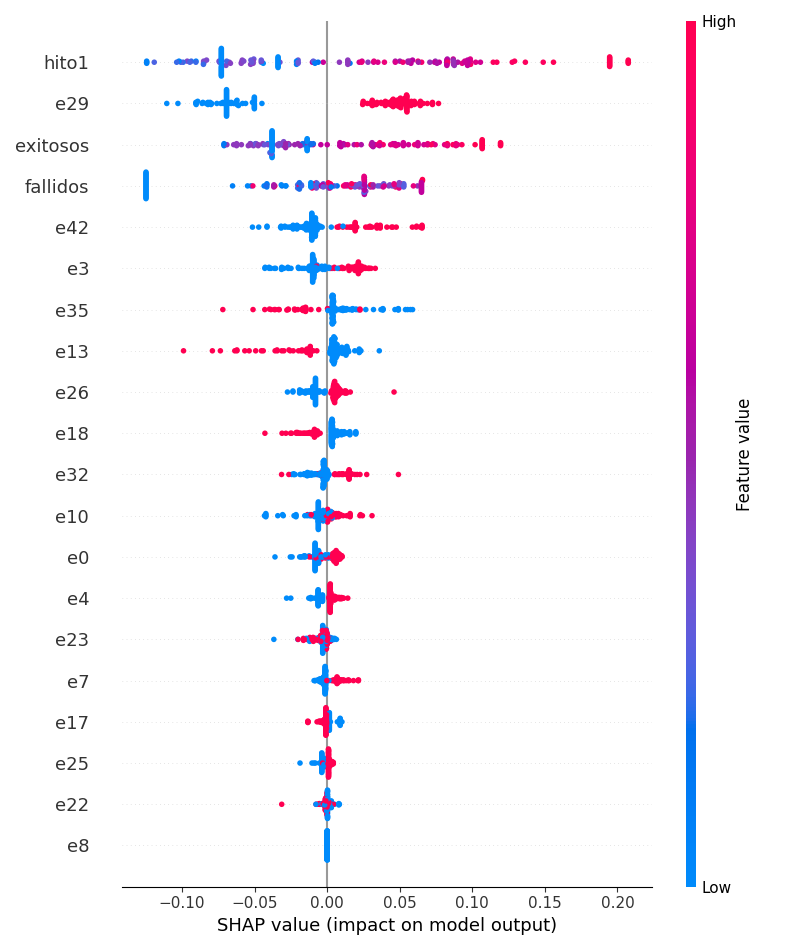
\includegraphics[width=6.0611in,height=6.6861in]{img/shap_rf/shapForcePlot2.png}
    \caption{Característica Variables SHAP}
    \label{fig:caract_var_shap}
\end{figure}

Podemos observar de forma breve que:

\say{hito1} tiene un alto impacto positivo acompañado de 
la pregunta de la guia \say{e29} tambien es una variable de interes de estudio, \say{exitosos} como \say{fallidos} tambien son variables muy interesantes de analisar, ya que estan correlacionadas con la intencion de resolver la guia.

por otro lado tenemos la figura de matplotlib

\begin{figure}[H]
    \centering
    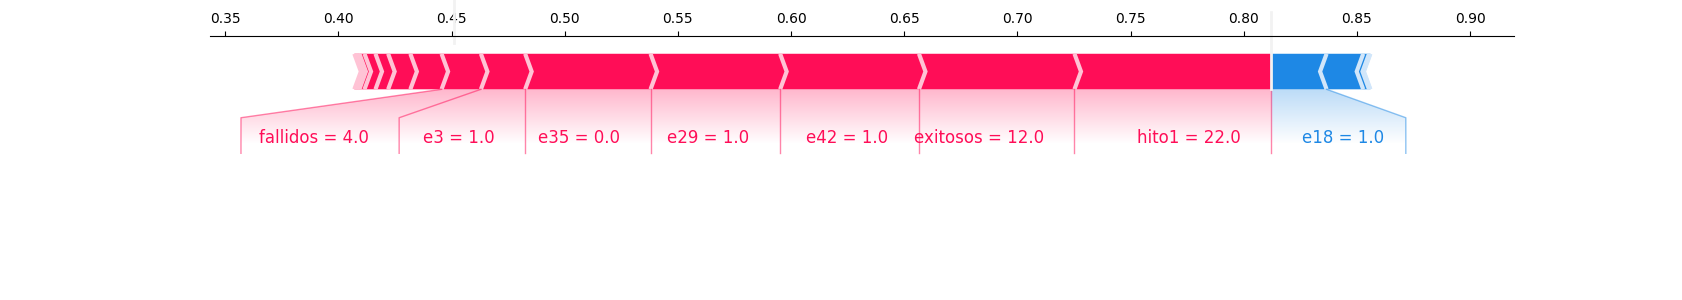
\includegraphics[width=6.0611in,height=1.6861in]{img/shap_rf/shapForcePlot.png}
    \caption{Característica Variables SHAP matplotlib}
    \label{fig:caract_var_shap_mat}
\end{figure}

Al revisar el grafico generado por matplotlib podemos ver:
+ hito1: con un 22.0 cumplido, tiene un 75\%  aproximandamente de importancia.
+ exitosos: tiene 12 respuestas y aproximadamente un 67\% de importancia.
+ e42: La variable tiene una respuesta de 1.0 en la pregunta de la guía y aproximadamente un 59\% de importancia.
+ e29: La variable tiene una respuesta de 1.0 en la pregunta de la guía y aproximadamente un 54\% de importancia.
+ e35: La variable tiene una respuesta de 1.0 en la pregunta de la guía y aproximadamente un 47\% de importancia.
+ e3: La variable tiene una respuesta de 1.0 en la pregunta de la guía y aproximadamente un 46\% de importancia.
+ fallidos: La variable tiene 4.0 intentos para lograr el éxito en la pregunta y aproximadamente un 49\% de importancia.

El impacto más bajo lo presenta la variable \say{e18}, con una respuesta de 1.0 en la pregunta de la guía y una importancia aproximada del 81\% al 85\%.

La marca \say{f(x)} en el gráfico representa el valor de predicción del modelo. En este caso, el valor es 0.81

Graficos de dependencia:

Representa la relación entre los valores de la variable \say{hito1}, say{e29}, say{exitosos},\say{fallidos}, \say{e42} y los valores de Shapley en el modelo. Proporciona una visualización de cómo las variable en cuestion influye en las predicciones del modelo y ayuda a entender su importancia relativa.

\begin{figure}[H]
    \centering
    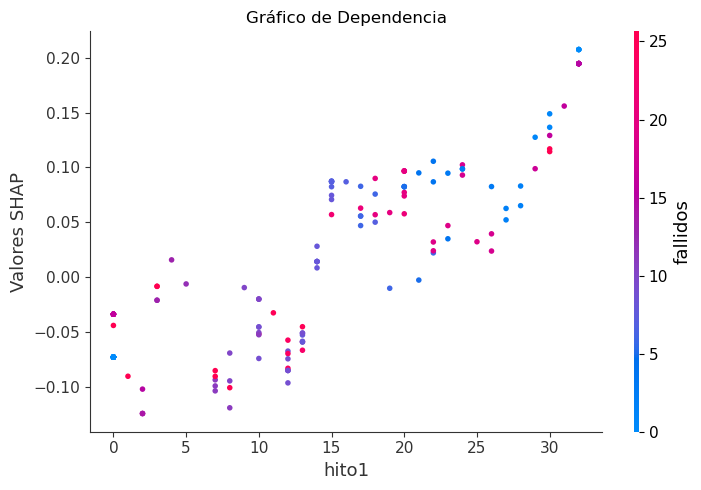
\includegraphics[width=4.0611in,height=2.6861in]{img/shap_rf/hito1.png}
    \caption{Variable dependencia hito1}
    \label{fig:dependencia_hito1}
\end{figure}

\begin{figure}[H]
    \centering
    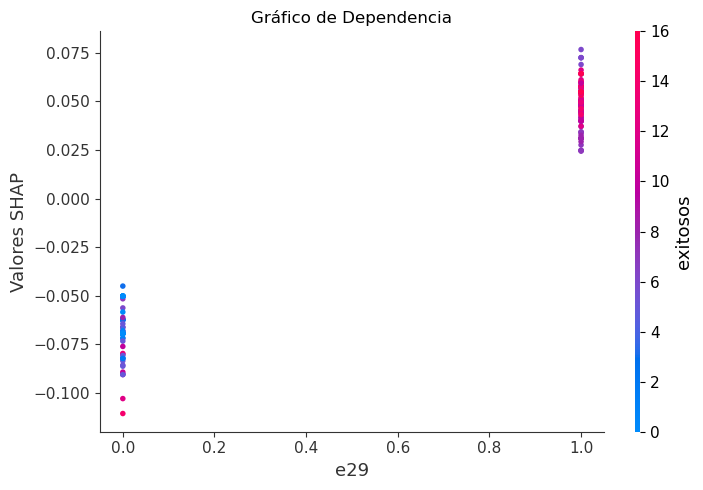
\includegraphics[width=4.0611in,height=2.6861in]{img/shap_rf/e29.png}
    \caption{Variable dependencia e29}
    \label{fig:dependencia_e29}
\end{figure}

\begin{figure}[H]
    \centering
    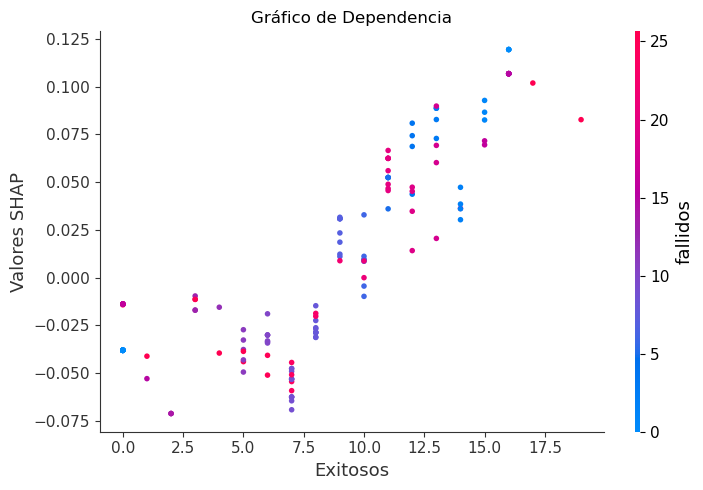
\includegraphics[width=4.0611in,height=2.6861in]{img/shap_rf/exitosos.png}
    \caption{Variable dependencia exitosos}
    \label{fig:dependencia_exitosos}
\end{figure}

\begin{figure}[H]
    \centering
    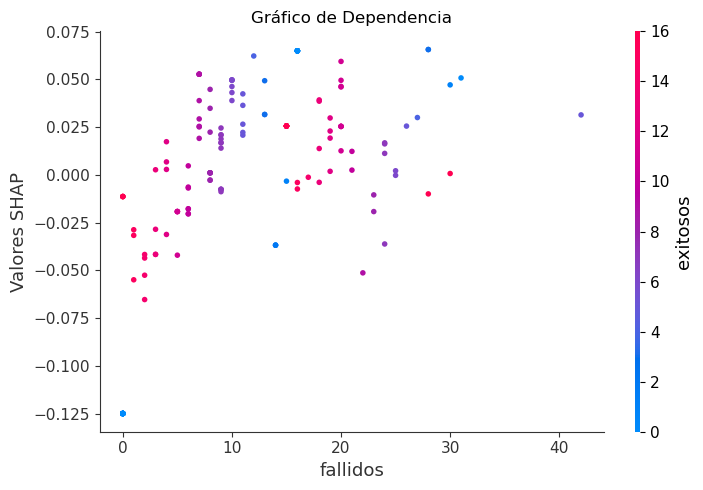
\includegraphics[width=4.0611in,height=2.6861in]{img/shap_rf/fallidos.png}
    \caption{Variable dependencia fallidos}
    \label{fig:dependencia_fallidos}
\end{figure}